\documentclass[border=10pt, tikz]{standalone}
\usetikzlibrary{arrows.meta, positioning, calc, patterns, decorations.markings}
\usepackage{amsmath, amssymb}

% Colors matching the blog's palette
\definecolor{interiorCol}{HTML}{0f85a5}  % Teal (interior derivative)
\definecolor{boundaryCol}{HTML}{e69138}  % Orange (boundary derivative)
\definecolor{emitBlue}{HTML}{5bc0de}     % Emitting patch 1
\definecolor{emitOrange}{HTML}{e67e22}   % Emitting patch 2
\definecolor{surfGray}{HTML}{d0d0d0}     % Surface fill
\definecolor{surfEdge}{HTML}{b0b0b0}     % Surface edge fill
\definecolor{tablehead}{HTML}{1a5276}    % Dark teal table header
\definecolor{tablealt}{HTML}{f0f4f8}     % Alternating row
\definecolor{textdark}{HTML}{222222}

\begin{document}
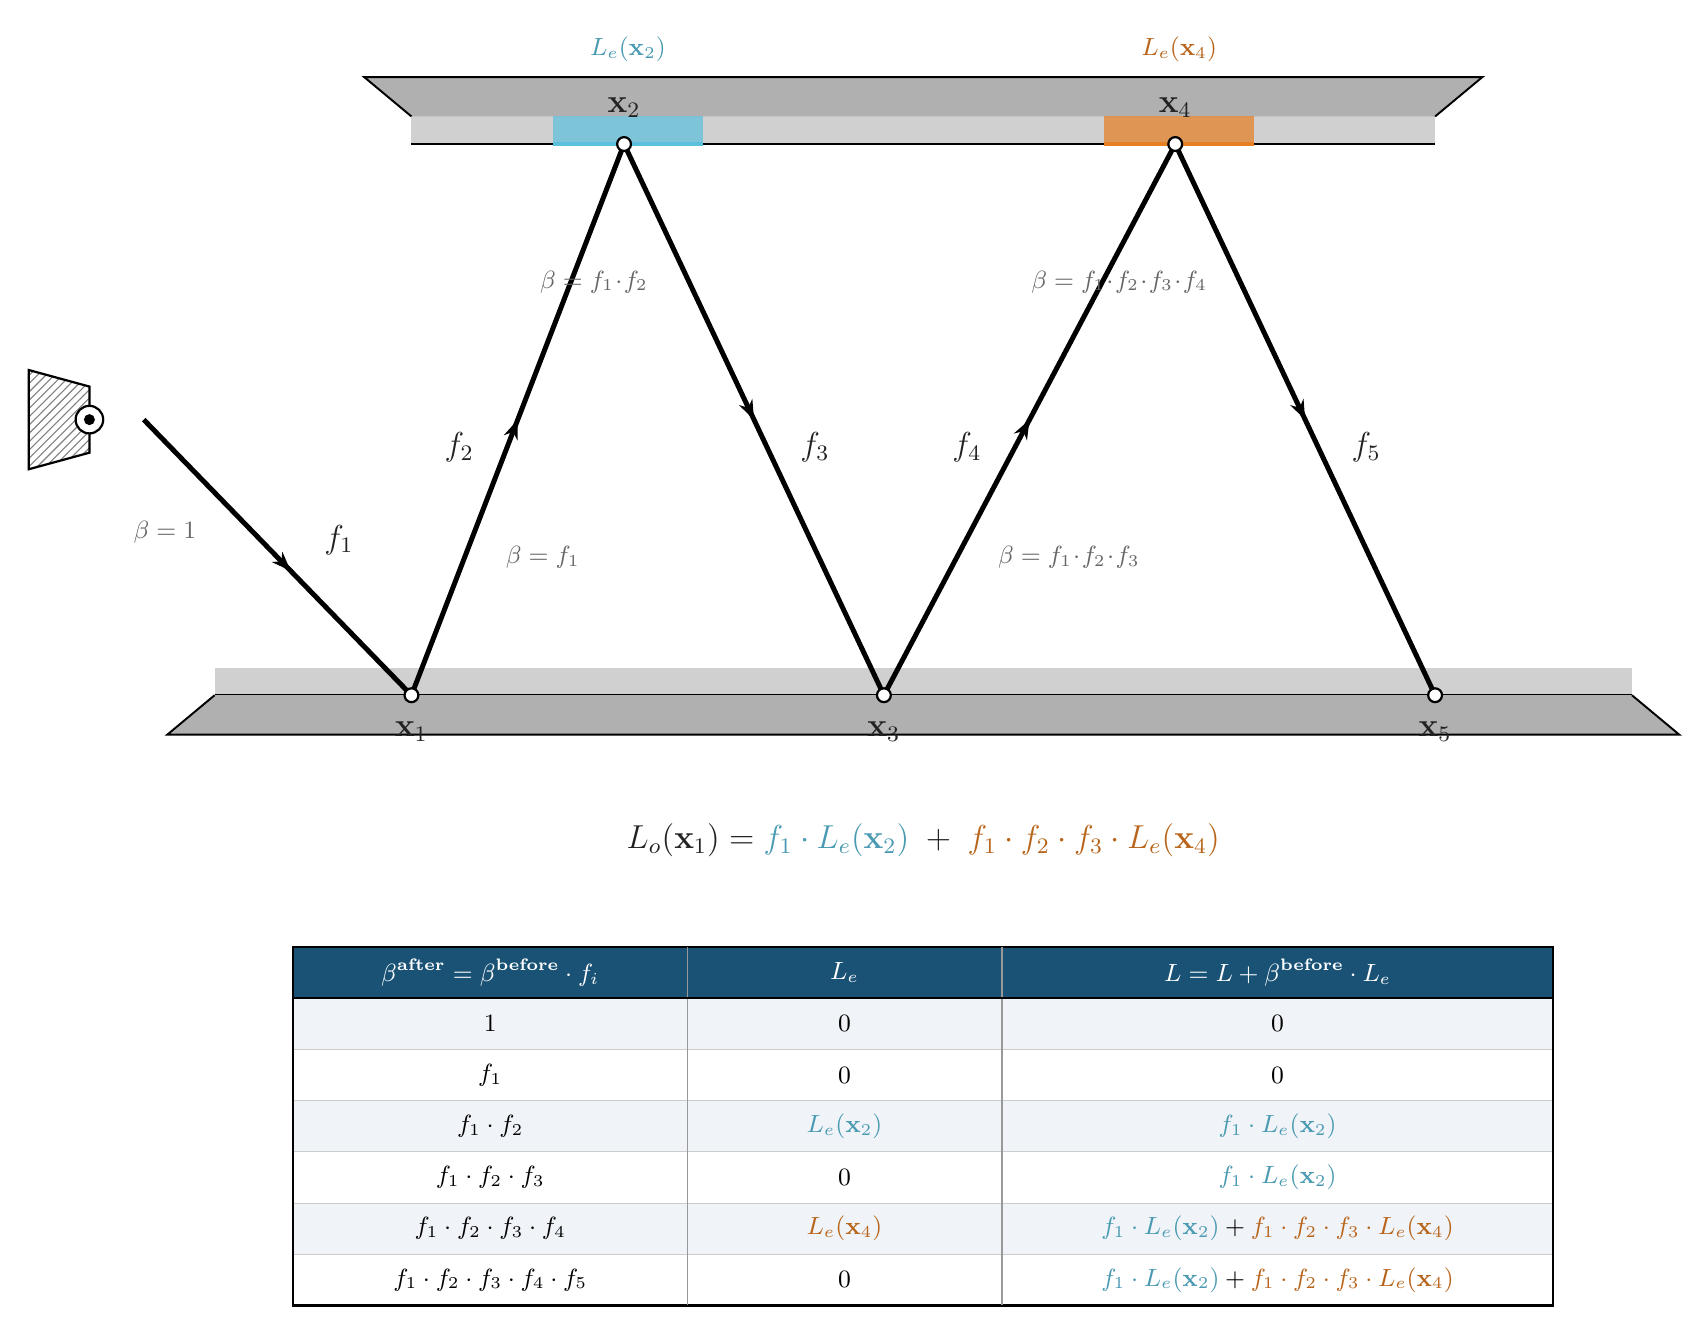
\begin{tikzpicture}[
    font=\sffamily,
    >=Stealth,
    vertex/.style={circle, draw=black, fill=white, inner sep=0pt, minimum size=5pt, line width=0.8pt},
    bsdf/.style={font=\large\bfseries, text=textdark},
    throughput/.style={font=\small, text=black!60},
    vlabel/.style={font=\large\bfseries, text=textdark},
]

% ============================================================
%  SCENE GEOMETRY
% ============================================================

% --- Floor surface (3D perspective) ---
\fill[surfGray] (0, 0) rectangle (18, 0.35);
\draw[black, line width=1pt] (0, 0) -- (18, 0);
\fill[surfEdge] (0, 0) -- (-0.6, -0.5) -- (18.6, -0.5) -- (18, 0) -- cycle;
\draw[black, line width=0.7pt] (0, 0) -- (-0.6, -0.5) -- (18.6, -0.5) -- (18, 0);

% --- Ceiling surface (3D perspective) ---
\fill[surfGray] (2.5, 7) rectangle (15.5, 7.35);
\draw[black, line width=1pt] (2.5, 7) -- (15.5, 7);
\fill[surfEdge] (2.5, 7.35) -- (1.9, 7.85) -- (16.1, 7.85) -- (15.5, 7.35) -- cycle;
\draw[black, line width=0.7pt] (2.5, 7.35) -- (1.9, 7.85) -- (16.1, 7.85) -- (15.5, 7.35);

% --- Emitting patches on ceiling ---
\fill[emitBlue, opacity=0.7] (4.3, 7) rectangle (6.2, 7.35);
\draw[emitBlue, line width=1.2pt] (4.3, 7) -- (6.2, 7);
\fill[emitOrange, opacity=0.7] (11.3, 7) rectangle (13.2, 7.35);
\draw[emitOrange, line width=1.2pt] (11.3, 7) -- (13.2, 7);

% ============================================================
%  CAMERA
% ============================================================
\begin{scope}[shift={(-1.8, 3.5)}, scale=0.7]
    % Camera body (hatched trapezoid)
    \fill[pattern=north east lines, pattern color=black!50, draw=black, line width=0.8pt]
        (-0.8, -0.9) -- (0.3, -0.6) -- (0.3, 0.6) -- (-0.8, 0.9) -- cycle;
    % Lens
    \draw[black, fill=white, line width=0.8pt] (0.3, 0) circle (0.25);
    \fill[black] (0.3, 0) circle (0.1);
\end{scope}

% ============================================================
%  VERTICES
% ============================================================
\coordinate (cam) at (-0.9, 3.5);
\coordinate (x1) at (2.5, 0);
\coordinate (x2) at (5.2, 7);
\coordinate (x3) at (8.5, 0);
\coordinate (x4) at (12.2, 7);
\coordinate (x5) at (15.5, 0);

% ============================================================
%  RAY PATHS (with arrows at midpoints)
% ============================================================
\draw[black, line width=1.8pt,
    decoration={markings, mark=at position 0.55 with {\arrow{Stealth[length=7pt]}}},
    postaction={decorate}]
    (cam) -- (x1);

\draw[black, line width=1.8pt,
    decoration={markings, mark=at position 0.5 with {\arrow{Stealth[length=7pt]}}},
    postaction={decorate}]
    (x1) -- (x2);

\draw[black, line width=1.8pt,
    decoration={markings, mark=at position 0.5 with {\arrow{Stealth[length=7pt]}}},
    postaction={decorate}]
    (x2) -- (x3);

\draw[black, line width=1.8pt,
    decoration={markings, mark=at position 0.5 with {\arrow{Stealth[length=7pt]}}},
    postaction={decorate}]
    (x3) -- (x4);

\draw[black, line width=1.8pt,
    decoration={markings, mark=at position 0.5 with {\arrow{Stealth[length=7pt]}}},
    postaction={decorate}]
    (x4) -- (x5);

% ============================================================
%  VERTEX DOTS AND LABELS
% ============================================================
\node[vertex] at (x1) {};
\node[vertex] at (x2) {};
\node[vertex] at (x3) {};
\node[vertex] at (x4) {};
\node[vertex] at (x5) {};

\node[vlabel, below=6pt] at (x1) {$\mathbf{x}_1$};
\node[vlabel, above=6pt] at (x2) {$\mathbf{x}_2$};
\node[vlabel, below=6pt] at (x3) {$\mathbf{x}_3$};
\node[vlabel, above=6pt] at (x4) {$\mathbf{x}_4$};
\node[vlabel, below=6pt] at (x5) {$\mathbf{x}_5$};

% ============================================================
%  BSDF LABELS (at each bounce)
% ============================================================
\node[bsdf, anchor=west] at ($(cam)!0.55!(x1) + (0.3, 0.4)$)  {$f_1$};
\node[bsdf, anchor=east] at ($(x1)!0.45!(x2) + (-0.3, 0.0)$)  {$f_2$};
\node[bsdf, anchor=west] at ($(x2)!0.55!(x3) + (0.3, 0.0)$)   {$f_3$};
\node[bsdf, anchor=east] at ($(x3)!0.45!(x4) + (-0.3, 0.0)$)  {$f_4$};
\node[bsdf, anchor=west] at ($(x4)!0.55!(x5) + (0.3, 0.0)$)   {$f_5$};

% ============================================================
%  THROUGHPUT LABELS (along each ray segment)
% ============================================================
\node[throughput, anchor=east] at ($(cam)!0.35!(x1) + (-0.4, -0.2)$) {$\beta = 1$};
\node[throughput, anchor=west] at ($(x1)!0.25!(x2) + (0.4, 0.0)$) {$\beta = f_1$};
\node[throughput, anchor=east] at ($(x2)!0.25!(x3) + (-0.4, 0.0)$) {$\beta = f_1 \!\cdot\! f_2$};
\node[throughput, anchor=west] at ($(x3)!0.25!(x4) + (0.4, 0.0)$) {$\beta = f_1 \!\cdot\! f_2 \!\cdot\! f_3$};
\node[throughput, anchor=east] at ($(x4)!0.25!(x5) + (-0.3, 0.0)$) {$\beta = f_1 \!\cdot\! f_2 \!\cdot\! f_3 \!\cdot\! f_4$};

% ============================================================
%  EMISSION LABELS ON PATCHES
% ============================================================
\node[font=\small\bfseries, text=emitBlue!80!black, above=2pt] at (5.25, 7.85) {$L_e(\mathbf{x}_2)$};
\node[font=\small\bfseries, text=emitOrange!80!black, above=2pt] at (12.25, 7.85) {$L_e(\mathbf{x}_4)$};

% ============================================================
%  RADIANCE EQUATION (below the scene)
% ============================================================
\node[font=\large, text=textdark, anchor=north] at (9, -1.5) {%
    $L_o(\mathbf{x}_1) = 
    {\color{emitBlue!80!black} f_1 \cdot L_e(\mathbf{x}_2)} 
    \;+\; 
    {\color{emitOrange!80!black} f_1 \cdot f_2 \cdot f_3 \cdot L_e(\mathbf{x}_4)}$
};

% ============================================================
%  ACCUMULATION TABLE
% ============================================================
\begin{scope}[shift={(1.0, -3.2)}]
    % Table dimensions
    \def\colA{0}      % β^after column start
    \def\colB{5.0}    % L_e column start
    \def\colC{9.0}    % L column start
    \def\colEnd{16.0} % table end
    \def\rowH{0.65}   % row height
    
    % Header row
    \fill[tablehead] (\colA, 0) rectangle (\colEnd, -\rowH);
    \node[font=\small\bfseries, text=white, anchor=center] at ({(\colA+\colB)/2}, {-\rowH/2}) 
        {$\beta^{\text{after}} = \beta^{\text{before}} \cdot f_i$};
    \node[font=\small\bfseries, text=white, anchor=center] at ({(\colB+\colC)/2}, {-\rowH/2}) 
        {$L_e$};
    \node[font=\small\bfseries, text=white, anchor=center] at ({(\colC+\colEnd)/2}, {-\rowH/2}) 
        {$L = L + \beta^{\text{before}} \cdot L_e$};
    
    % Data rows
    \foreach \i/\betaval/\leval/\lval/\altfill in {
        1/{1}/{0}/{0}/{tablealt},
        2/{$f_1$}/{0}/{0}/{white},
        3/{$f_1 \cdot f_2$}/{\color{emitBlue!80!black}$L_e(\mathbf{x}_2)$}/{\color{emitBlue!80!black}$f_1 \cdot L_e(\mathbf{x}_2)$}/{tablealt},
        4/{$f_1 \cdot f_2 \cdot f_3$}/{0}/{\color{emitBlue!80!black}$f_1 \cdot L_e(\mathbf{x}_2)$}/{white},
        5/{$f_1 \cdot f_2 \cdot f_3 \cdot f_4$}/{\color{emitOrange!80!black}$L_e(\mathbf{x}_4)$}/{${\color{emitBlue!80!black}f_1 \cdot L_e(\mathbf{x}_2)} + {\color{emitOrange!80!black}f_1 \cdot f_2 \cdot f_3 \cdot L_e(\mathbf{x}_4)}$}/{tablealt},
        6/{$f_1 \cdot f_2 \cdot f_3 \cdot f_4 \cdot f_5$}/{0}/{${\color{emitBlue!80!black}f_1 \cdot L_e(\mathbf{x}_2)} + {\color{emitOrange!80!black}f_1 \cdot f_2 \cdot f_3 \cdot L_e(\mathbf{x}_4)}$}/{white}%
    } {
        \pgfmathsetmacro{\ystart}{-\i * \rowH}
        \fill[\altfill] (\colA, \ystart) rectangle (\colEnd, {\ystart - \rowH});
        \draw[black!20] (\colA, \ystart) -- (\colEnd, \ystart);
        \node[font=\small, anchor=center] at ({(\colA+\colB)/2}, {\ystart - \rowH/2}) {\betaval};
        \node[font=\small, anchor=center] at ({(\colB+\colC)/2}, {\ystart - \rowH/2}) {\leval};
        \node[font=\small, anchor=center] at ({(\colC+\colEnd)/2}, {\ystart - \rowH/2}) {\lval};
    }
    
    % Table border and column lines
    \draw[black, line width=0.8pt] (\colA, 0) rectangle (\colEnd, {-7*\rowH});
    \draw[black!40] (\colB, 0) -- (\colB, {-7*\rowH});
    \draw[black!40] (\colC, 0) -- (\colC, {-7*\rowH});
    \draw[black, line width=0.8pt] (\colA, -\rowH) -- (\colEnd, -\rowH);
\end{scope}

\end{tikzpicture}
\end{document}
